\documentclass{article}

\usepackage{amsmath}
\usepackage{amsfonts}
\usepackage{amsthm}
\usepackage{dynkin-diagrams}
\usepackage{algorithm2e}
\usepackage{enumerate}
\usepackage{tikz}
\usepackage[outline]{contour}
\contourlength{1.3pt}

% add shell-escape to commands
\usetikzlibrary{knots, cd, external, calc}
\tikzexternalize[prefix=tikz/]

\newtheorem{theorem}{Theorem}[section]
\newtheorem{corollary}[theorem]{Corollary}
\newtheorem{lemma}[theorem]{Lemma}
\newtheorem{question}[theorem]{Question}
\newtheorem{proposition}[theorem]{Proposition}
\newtheorem{problem}[theorem]{Problem}
\newtheorem{conjecture}[theorem]{Conjecture}

\theoremstyle{definition}
\newtheorem{examples}[theorem]{Examples}
\newtheorem{example}[theorem]{Example}
\newtheorem{notation}[theorem]{Notation}


\begin{document}

\begin{titlepage}
\begin{center}
\pagenumbering{gobble}
\Large{Department of Mathematics \\ of the University of Bern}\\
\vspace*{3.5cm}
\Huge{\textbf{Coxeter Quotients \\ of Link Groups}}\\
\vspace*{6.5cm}
\Large{Master Thesis of} \\ \Large{\textbf{Levi Ryffel}}\\
\vspace*{.25cm}
Supervised by \\ \textbf{Prof. Dr. Sebastian Baader}\\
\vspace*{2cm}
February 2020
\end{center}
\end{titlepage}
\pagenumbering{arabic}

\tableofcontents
\newpage

\section{Coxeter Groups}
\subsection{Coxeter Matrices and Graphs}
Let $S$ be a finite set and let $M = (m_{st})$ be an $S \times S$ matrix with coefficients in the set $\mathbb{N} \cup \{\infty\}$ satisfying $m_{ss} = 1$ for all $s \in S$, and $m_{st} \geq 2$ if $s \ne t$. Such a matrix is called a \textit{Coxeter matrix}. Consider the group presentation
$$W(M) = \langle S \; | \; (st)^{m_{st}} = 1 \text{ for } s,t\in S \rangle,$$
where we do not include relations of the form $(st)^\infty = 1$.
Then the group $W(M)$ is called the \textit{Coxeter group} corresponding to $M$. The tuple $(W(M),S)$ is called a \textit{Coxeter system} and the cardinality $\#S$ is referred to as its \textit{rank}. Since for us Coxeter groups always arise with a generating set, we blur the distinction between Coxeter groups and Coxeter systems.

Another way to encode the coefficients $m_{st}$ is to use them as weights in weighted undirected graphs, so-called \textit{Coxeter graphs}. In this case, the nodes of the graph are the generators, and the weight between the nodes $s$ and $t$ is $m_{st}$. The following shorthand notations are very common: If $m_{st} = 2$, then the edge between $s$ and $t$ is omitted and if $m_{st} = 3$, then the weight on the edge between $s$ and $t$ is omitted.

\begin{example}[Dihedral Groups]
The symmetry group of a regular $n$-gon is called the \textit{dihedral group} of order $2n$, denoted by the symbol $D_n$. This group is generated by two reflections $s, t$ whose composition is a rotation by an angle of~$2\pi/n$. This is used to show that $D_n$ is isomorphic to the Coxeter group
$$W = \langle s, t \; | \; (st)^n = s^2 = t^2 = 1 \rangle.$$
Thus, Coxeter groups on two generators whose product has finite order are dihedral groups.

This observation is often used to motivate the introduction of one more dihedral group, the so-called \textit{infinite dihedral group} with presentation
$$D_\infty = \langle s, t \; | \; s^2 = t^2 = 1 \rangle.$$
\end{example}
\subsection{The Reflection Representation}
A well-known construction leading to an easy solution of the word-problem for Coxeter groups and also helping in adapting a geometric viewpoint to the study of Coxeter groups is a faithful representation of any Coxeter group where its generating sets acts as a set of reflections with respect to a (possibly degenerate) bilinear form.

Let $(W,S)$ be a Coxeter system, and let $n = \#S$. Then we consider the bilinear form on $\mathbb{R}^S$ given by the matrix $B = (b_{st})$ with entries $b_{st} = -\cos \pi/m_{st}$. 
For $s \in S$ let $\rho_s$ be the \textit{reflection} with respect to $B$ with root $e_s \in \mathbb{R}^n$ given by the formula
$$ \rho_s(x) = x - 2B(x, e_s)e_s,$$
where $x \in \mathbb{R}^S$.

\begin{proposition}\label{prop:reflection-representation-well-defined}
Let $(W,S)$ be a Coxeter system and let $s, t \in S$. Then the reflections $\rho_s$ and $\rho_t$ satisfy $(\rho_s \rho_t)^{m_{st}} = 1$.
\end{proposition}

\begin{proof}
First of all, observe that each reflection $\rho_s$ fixes an $(n-1)$-dimensional hyperplane, namely the orthogonal complement of the non-isotropic vector $e_s$. Now fix $s,t\in S$ and consider the subspace $V_{st} = \mathbb{R}e_s \oplus \mathbb{R}e_t$, which is invariant under $\rho_s$ and $\rho_t$. Since the orthogonal complement of $V_{st}$ is fixed by $\rho_s$ and $\rho_t$, the order of $\rho_s\rho_t$ on $\mathbb{R}^S$ is equal to its order on $V_{st}$.

Let us now distinguish two cases. If $m_{st}$ is finite, $B$ restricted to $V_{st}$ is positive definite. To see this, consider an arbitrary vector $v = ae_s + b e_t$ in $V_{st}$ and compute
\begin{align*}
B(v, v) & = a^2B(e_s, e_s) + 2abB(e_s, e_t) + b^2B(e_t, e_t)\\
& = a^2 + 2ab\text{cos } -\pi / m_{st} + b^2 \\
& > a^2 - 2ab + b^2 = (a - b)^2 > 0.
\end{align*}
Thus, $V_{st}$ is isometric to $\mathbb{R}^2$ with the standard inner product, and the angle between the invariant subspaces of $\rho_s$ and $\rho_t$ is equal to $2 \pi / m_{st}$. This shows that $\rho_s$ and $\rho_t$ are symmetries of a regular $n$-gon and their product is a rotation by $2\pi/m_{st}$, which has order $m_{st}$.

On the other hand, if $m_{st} = \infty$ the matrix of $\rho_s\rho_t$ is given by
$$\rho_s \rho_t = \left( \begin{matrix}
-1 & 1 \\ 1 & -1
\end{matrix} \right)
\left( \begin{matrix}
1 & -1 \\ -1 & 1
\end{matrix} \right)
= \left( \begin{matrix}
0 & 2 \\ 2 & 0
\end{matrix} \right)
$$
which has infinite order.
\end{proof}

This shows that the map $s \mapsto \rho_s$ induces a representation of $W$, called the \textit{reflection representation} of $W$. We will conclude this section by showing that this representation is faithful. But first we need some preparation.

To any Coxeter group $W$ we can assign a \textit{length function} $l: W \rightarrow \mathbb{N}$, assigning to any element $w$ of $W$ the minimal number of generating reflections needed to write down an expression for $w$. An expression for $w$ of length $l(w)$ is called a \textit{reduced expression} for $w$.

To get a little bit of a feeling how the length function behaves for Coxeter groups (or more generally, for groups generated by elements of order two subject only to relations of even length, such as the reflection quotient from Section \ref{subsec:reflection-quotient}), we prove the following illustrative result.

\begin{proposition}
Let $W$ be a Coxeter group, $w \in W$ and $s \in S$. Then either $l(ws) = l(w) + 1$ or $l(ws) = l(w) - 1$.
\end{proposition}

\begin{proof}
First of all, we make the obvious observation that for any words 
$w, w' \in W$ we have that $l(ww') \leq l(w) + l(w')$. This immediately implies that $l(ww') \geq l(w) - l(w')$ by applying the above to the pair $ww'$ and $w'^{-1}$ instead of $w$ and $w'$, observing that $l(w) = l(w^{-1})$ for all $w \in W$. We conclude that
$$l(w) - 1 \leq l(ws) \leq l(w) + 1.$$
The only thing left to show is that in fact $l(ws) \neq l(w)$. To see this, we introduce the \textit{sign} homomorphism $\varepsilon: W \rightarrow \{\pm 1\}$ defined via $s \mapsto -1$ for all $s \in S$. Indeed, this extends to $W$ since all relations of $W$ are of even length. Obviously we have $\varepsilon(w) = (-1)^{l(w)}$, and $\varepsilon(ws) \neq \varepsilon(w)$. This implies that $l(ws) \neq l(w)$, which is precisely what we wanted to show.
\end{proof}

For a vector $v$ in $\mathbb{R}^S$ we will write $v > 0$ if $v$ is non-zero and is a non-negative linear combination of the $e_s$. Moreover, $v < 0$ if $-v>0$. This enables us to formulate the following important Lemma. A consequence of it that is easy to formulate and captures its essence goes as follows: Whenever $we_s$ lies in the positive cone, that is $w e_s > 0$, then $w$ does not have a reduced expression ending in $s$. Be warned that although the converse is true, it does not immediately follow.

\begin{lemma}\label{lem:humphreys5.4}
Let $W$ be a Coxeter group, $w \in W$ and $s \in S$. Then $we_s > 0$ if and only if $l(ws) = l(w) + 1$.
\end{lemma}

\begin{proof}
This is taken from \cite{humphreys1990}. Note first that it suffices to prove that whenever $l(ws) = l(w) + 1$ we have that $we_s > 0$, since applying this to $ws$ instead of $w$ proves its converse. 

The proof of this direction is a proof by induction on $l(w)$. Suppose $l(w) = 0$. Then $w$ is the identity and $l(ws) = l(w) + 1$ for all $s$. 

For the inductive step, Let $t$ be any reflection in $S$ such that $l(wt) = l(w) - 1$, taking for example $t$ to be the last symbol in a reduced expression for $w$. Write $w = w'w_{st}$, where $w_{st}$ is a word in the symbols $s, t$ of maximal length such that the length of the expression $w'w_{st}$ is equal to $l(w)$. This exists since $w_{st}$ equal to the empty word is in fact a (non-maximal) solution.

We will now prove the Lemma by showing that $w'e_s > 0$, $w'e_t > 0$ and $w_{st}e_s > 0$, and that $w_{st}$ is non-empty. Taking $w_{st} = t$ shows that $l(w') < l(w)$, so we can apply the induction hypothesis to $w'$, showing that $w'e_s > 0$ and $w'e_t > 0$ provided we can show that $l(w's) > l(w')$ and $l(w't) > l(w')$. 

Suppose toward a contradiction that $l(w's) < l(w')$. Then $sw_{st}$ is in fact a longer word than $w_{st}$, contradicting maximality of $w_{st}$. Similarly it is also true that $l(w't) > l(w')$.

Finally we draw a picture to show that $v_{st}e_s > 0$. Note first that $v_{st}$ does not have a reduced expression ending in $s$, since if it did we would actually reduce its length by adding an $s$ to the end. In particular, the length of $w_{st}$ is strictly less than $m_{st}$, that is, interpreting $w_{st}$ as a map on the plane as in the proof of Proposition \ref{prop:reflection-representation-well-defined}, $w_{st}$ is not rotation by an angle of $\pi$. 

\begin{figure}
\centering
\begin{minipage}{.5\textwidth}
\centering
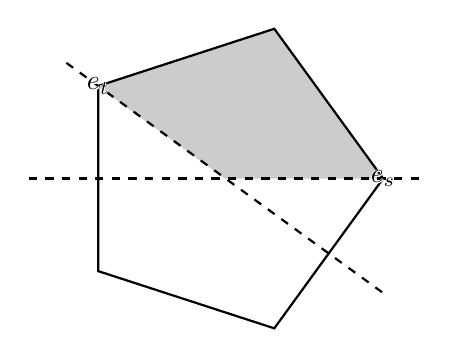
\begin{tikzpicture}[scale = 0.5]
% pentagon
\filldraw[color = black!20] (4, 0) -- (72:4) -- (144:4) -- (0, 0);
\draw[thick] (4, 0) -- (72:4) -- (144:4) -- (216:4) -- (288:4) -- (4, 0);
\draw[thick, dashed] (-5, 0) -- (5, 0);
\draw[thick, dashed] (144:5) -- (144:-5);

\node at (4, 0) {\contour{white}{$e_s$}};
\node at (144:4) {\contour{white}{$e_t$}};

\end{tikzpicture}
\end{minipage}%
\begin{minipage}{.5\textwidth}
\centering

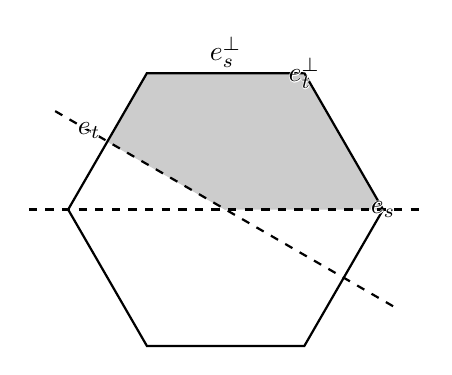
\begin{tikzpicture}[scale = 0.5]
% hexagon
\filldraw[color = black!20] (4, 0) -- (60:4) -- (120:4) -- ($(120:4)!0.5!(180:4)$) -- (0, 0);
\draw[thick] (4, 0) -- (60:4) -- (120:4) -- (180:4) -- (60:-4) -- (120:-4) -- (4, 0);

\draw[thick, dashed] (-5, 0) -- (5, 0);
\draw[thick, dashed] (150:5) -- (150:-5);

\node at (4, 0) {\contour{white}{$e_s$}};
\node at (150:4) {\contour{white}{$e_t$}};
\node at (60:4) {\contour{white}{$e_t^{\perp}$}};
\node at (90:4) {\contour{white}{$e_s^\perp$}};

\end{tikzpicture}
\end{minipage}
\caption{Illustration of the fact that $e_s$ lands in the positive cone, indicated in grey.}
\end{figure}
\end{proof}

\begin{theorem}
The reflection representation is faithful.
\end{theorem}

\begin{proof}
Suppose $w$ lies in the kernel of the reflection representation. Then obviously $we_s > 0$ for all $s \in S$, so by Lemma \ref{lem:humphreys5.4}, $l(ws) = l(w) + 1$ for all $s \in S$, i.e., for any $s \in S$ we have that $w$ does not have a reduced expression ending in $s$. But this implies that $w$ is the identity.
\end{proof}

\subsection{The Word Problem}
In this section we study an alternative solution to the word problem in Coxeter groups due to Tits. %TODO cite
\begin{notation}
Let $W$ be a Coxeter group with generating set $S$ and Coxeter matrix $M = (m_{st})$. Then we agree on the convention that
$$(st)^{m_{st}/2} =  \begin{cases}
(st)^k & \text{ if } m_{st} = 2k, \\
(st)^ls & \text{ if } m_{st} = 2l + 1.
\end{cases}$$
E.g., if $m_{st}=5$ we write $(st)^{5/2} = ststs$. 
\end{notation}

%TODO cite properly
\begin{theorem}[Tits]\label{thm:word-problem}
Let $F$ be the free monoid generated by the set $S$. Suppose the word $w \in F$ represents the trivial element in a Coxeter group $W$ with generating set $S$ and Coxeter matrix $M = (m_{st})$. Then there is a sequence of moves of the following two types carrying $w$ to the empty word.

\begin{enumerate}[\textup{(}i\textup{)}]
\item removing occurrences of $s^2$ from $w$ for $s \in S$.
\item replacing occurrences of $(st)^{m_{st}/2}$ by $(ts)^{m_{st}/2}$ for $s, t \in S$.
\end{enumerate}
\end{theorem}

\subsection{Finite Coxeter Groups}

\newpage

\section{Knot Theory}
\subsection{Knots and Links}
A \textit{knot} $K$ is the image of a smooth embedding of $S^1$ into $S^3$. A \textit{link} $L$ is a disjoint union of finitely many knots. Two links $L \subset S^3$ and $L' \subset S^3$ are said to be \textit{equivalent} if there exists a diffeomorphism between the pair $(S^3, L)$ and the pair $(S^3, L')$, i.e., a diffeomorphism $S^3 \rightarrow S^3$ that restricts to a diffeomorphism of the links $L \rightarrow L'$.

\begin{example}[Torus Links]
Let $p, q$ be integers. Consider the universal covering $\mathbb{R}^2 \rightarrow T^2$, where $T^2 \subset \mathbb{R}^3$ is a standardly embedded torus (consider e.g. Example 6 of Section 2-2 in \cite{docarmo1976}). Then the $(p,q)$-\textit{torus link} is the image of the lines through $\mathbb{Z}e_1$ of slope $p/q$.
\end{example}

\begin{example}[Pretzel Links]
The $(l_1, \dots, l_k)$-\textit{Pretzel link} is the link obtained by connecting 2-braids in the way indicated in Figure \ref{fig:pretzel-link}.
%TODO introduce 2-braids

\begin{figure}[ht]
\centering
\begin{minipage}{0.5\textwidth}
\centering
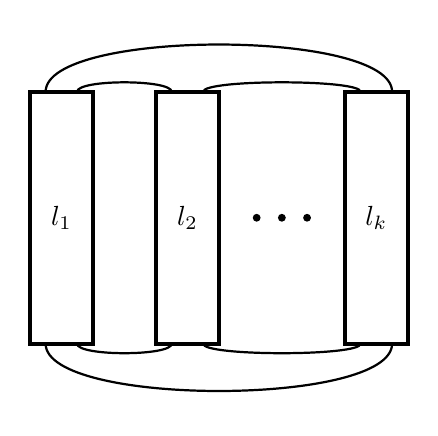
\begin{tikzpicture}[scale = 0.8]
\draw[ultra thick] (0, 0) rectangle (1,4);
\draw[ultra thick] (2, 0) rectangle (3, 4);
\node at (3.6, 2) [circle, fill, inner sep=1pt] {};
\node at (4,2) [circle, fill, inner sep=1pt] {};
\node at (4.4, 2) [circle, fill, inner sep=1pt] {};
\draw[ultra thick] (5, 0) rectangle (6, 4);

\begin{knot}
\strand[thick] (0.25, 4) .. controls +(0, 1) and +(0, 1) .. (5.75, 4);
\strand[thick] (0.75, 4) .. controls +(0, 0.2) and +(0, 0.2) .. (2.25, 4);
\strand[thick] (2.75, 4) .. controls +(0, 0.2) and +(0, 0.2) .. (5.25, 4);

\strand[thick] (0.25, 0) .. controls +(0, -1) and +(0, -1) .. (5.75, 0);
\strand[thick] (0.75, 0) .. controls +(0, -0.2) and +(0, -0.2) .. (2.25, 0);
\strand[thick] (2.75, 0) .. controls +(0, -0.2) and +(0, -0.2) .. (5.25, 0);
\end{knot}

\node at (0.5, 2) {$l_1$};
\node at (2.5, 2) {$l_2$};
\node at (5.5, 2) {$l_k$};

\end{tikzpicture}
\caption{$P(l_1, l_2, \dots, l_k)$}
\label{fig:pretzel-link}
\end{minipage}%
\begin{minipage}{0.5\textwidth}
\centering
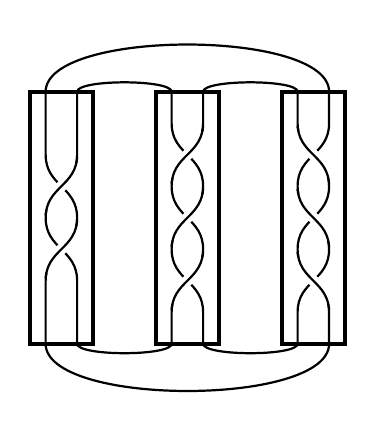
\begin{tikzpicture}[scale = 0.8]

\draw[ultra thick] (0, -0.5) rectangle (1, 3.5);
\draw[ultra thick] (2, -0.5) rectangle (3, 3.5);
\draw[ultra thick] (4, -0.5) rectangle (5, 3.5);

\begin{knot}[clip width = 5, flip crossing/.list={2, 4, 6, 8}]
\strand[thick] (0.25, -0.5) -- (0.25, 0.5) .. controls +(0, 0.5) and +(0, -0.5) .. (0.75, 1.5) .. controls +(0, 0.5) and +(0, -0.5) .. (0.25, 2.5) -- (0.25, 3.5);

\strand[thick] (0.75, -0.5) -- (0.75, 0.5) .. controls +(0, 0.5) and +(0, -0.5) .. (0.25, 1.5) .. controls +(0, 0.5) and +(0, -0.5) .. (0.75, 2.5) -- (0.75, 3.5);


\strand[thick] (2.25, -0.5) -- (2.25, 0) .. controls +(0, 0.5) and +(0, -0.5) .. (2.75, 1) .. controls +(0, 0.5) and +(0, -0.5) .. (2.25, 2) .. controls +(0, 0.5) and +(0, -0.5) .. (2.75, 3) -- (2.75, 3.5);

\strand[thick] (2.75, -0.5) -- (2.75, 0) .. controls +(0, 0.5) and +(0, -0.5) .. (2.25, 1) .. controls +(0, 0.5) and +(0, -0.5) .. (2.75, 2) .. controls +(0, 0.5) and +(0, -0.5) .. (2.25, 3) -- (2.25, 3.5);



\strand[thick] (4.25, -0.5) -- (4.25, 0) .. controls +(0, 0.5) and +(0, -0.5) .. (4.75, 1) .. controls +(0, 0.5) and +(0, -0.5) .. (4.25, 2) .. controls +(0, 0.5) and +(0, -0.5) .. (4.75, 3) -- (4.75, 3.5);

\strand[thick] (4.75, -0.5) -- (4.75, 0) .. controls +(0, 0.5) and +(0, -0.5) .. (4.25, 1) .. controls +(0, 0.5) and +(0, -0.5) .. (4.75, 2) .. controls +(0, 0.5) and +(0, -0.5) .. (4.25, 3) -- (4.25, 3.5);

\strand[thick] (0.75, -0.5) .. controls +(0, -0.2) and +(0, -0.2) .. (2.25, -0.5);
\strand[thick] (2.75, -0.5) .. controls +(0, -0.2) and +(0, -0.2) .. (4.25, -0.5);
\strand[thick] (0.25, -0.5) .. controls +(0, -1) and +(0, -1) .. (4.75, -0.5);


\strand[thick] (0.75, 3.5) .. controls +(0, 0.2) and +(0, 0.2) .. (2.25, 3.5);
\strand[thick] (2.75, 3.5) .. controls +(0, 0.2) and +(0, 0.2) .. (4.25, 3.5);
\strand[thick] (0.25, 3.5) .. controls +(0, 1) and +(0, 1) .. (4.75, 3.5);


\end{knot}
\end{tikzpicture}
\caption{$P(2, 3, -3)$}
\end{minipage}
\end{figure}
\end{example}
\subsection{The Bridge Index}
Let $L \subset S^3$ be a link. The minimal number of local maxima of a smooth function $S^3 \rightarrow \mathbb{R}$ restricted to $L$ is called the \textit{bridge index} of $L$ and referred to as $\text{bi } L$.

This can be diagrammatically characterized in the following way. Let $D$ be a diagram of $L$. An \textit{arc} in $D$ is a segment of $D$ beginning and ending with an undercrossing, containing no undercrossings in between. A \textit{bridge} of $D$ is an arc of $D$ that contains at least one overcrossing.

\begin{proposition}
The bridge index of a link $L \subset S^3$ is equal to the number of bridges in a diagram $D$ of $L$, minimized over all diagrams.
\end{proposition}

%TODO prove or cite

\begin{proposition}\label{prop:bridge-index-connected-sum}
Let $K$ and $K'$ be knots. Then $\textup{bi } K\#K' = \textup{bi } K + \textup{bi }K' - 1$.
\end{proposition}

\subsection{The Alexander Polynomial}
\subsection{The Link Group}\label{subsec:link-group}
The \textit{link group} of a link $L \subset S^3$ is $\pi(L) = \pi_1(S^3 \setminus L)$. If $L$ is a knot $K$ then the link group $\pi(K)$ is referred to as its \textit{knot group}.

The knot group essentially classifies all knots, in that if two knots have isomorphic knot groups then they are equivalent. Be warned that this is no longer true for links, see \cite{rolfsen2003}. This suggests that studying the knot group might be just as good as studying knots themselves.

We will now describe an algorithm that computes the link group of an oriented link. Let $L \subset S^3$ be a link and let $D$ be any diagram of $L$. Let $S = \{m_1, \dots, m_k\}$ be the set of diagram meridians, oriented from right to left. A meridian $m_i$ should be interpreted at as the meridian starting at the reader's eye, passing under the arc and going back to the reader's eye without any detour.

Having assigned a generator to every crossing, we now assign a relator $r$ to any crossing, as indicated in Figure \ref{fig:wirtinger-relations}.

\begin{figure}[h]
\centering
\begin{minipage}{.5\textwidth}
\centering
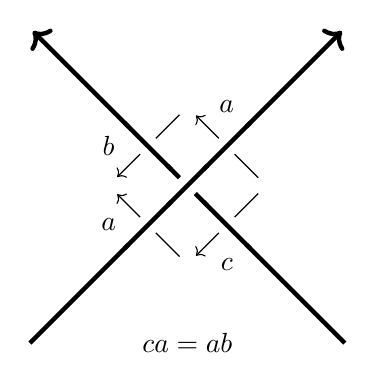
\begin{tikzpicture}
\begin{knot}[clip width = 5]
\strand[black, ultra thick, ->] (0, 0) -- (4, 4);
\strand[black, ultra thick, ->] (4, 0) -- (0, 4);

\strand[black, ->] (1.9, 1.1) -- (1.1, 1.9);
\strand[black, ->] (1.9, 2.9) -- (1.1, 2.1);
\strand[black, ->] (2.9, 2.1) -- (2.1, 2.9);
\strand[black, ->] (2.9, 1.9) -- (2.1, 1.1);

\node at (1, 1.5) {$a$};
\node at (1, 2.5) {$b$};
\node at (2.5, 3) {$a$};
\node at (2.5, 1) {$c$};

\node at (2, 0) {$ca = ab$};
\end{knot}
\end{tikzpicture}
\end{minipage}%
\begin{minipage}{.5\textwidth}
\centering
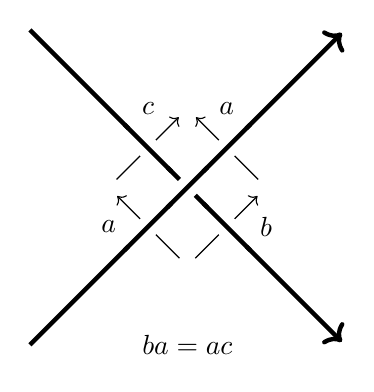
\begin{tikzpicture}
\begin{knot}[clip width = 5]
\strand[black, ultra thick, ->] (0, 0) -- (4, 4);
\strand[black, ultra thick, ->] (0, 4) -- (4, 0);

\strand[black, ->] (1.9, 1.1) -- (1.1, 1.9);
\strand[black, ->] (1.1, 2.1) -- (1.9, 2.9);
\strand[black, ->] (2.9, 2.1) -- (2.1, 2.9);
\strand[black, ->] (2.1, 1.1) -- (2.9, 1.9);

\node at (1, 1.5) {$a$};
\node at (1.5, 3) {$c$};
\node at (2.5, 3) {$a$};
\node at (3, 1.5) {$b$};

\node at (2, 0) {$ba = ac$};
\end{knot}
\end{tikzpicture}
\end{minipage}
\caption{Relations in the Wirtinger Presentation}
\label{fig:wirtinger-relations}
\end{figure}

The fact that the resulting presentation is actually a presentation for the link group of $L$ is a Seifert-van Kampen argument, elaborated upon for example in \cite{rolfsen2003}.

\newpage

\section{Coxeter Quotients}
\subsection{The Reflection Quotient}\label{subsec:reflection-quotient}
Let $L \subset S^3$ be a link. A \textit{Coxeter quotient} is a quotient $\pi(K)/N$ of the link group which is isomorphic to a Coxeter group $W(M)$ such that every meridian in $\pi(L)$ corresponds to a reflection in $W(M)$.

In many cases, finding Coxeter quotients of links is rather straight-forward, at least with the help of a computer. This is because checking whether a specific set of Coxeter relations induces a Coxeter quotient of a link amounts to checking the validity of the defining relations in its link group.

The \textit{reflection quotient} is the group $r(L) = \pi_1(S^3 \setminus L) / \langle \langle m^2 \rangle \rangle$, where $m$ is any meridian of $L$. Because it is clumsy to write down a presentation in this fashion we agree to add the relations $s^2$ for all $s \in S$ when writing a presentation as $\langle S \; | \; R \rangle^{(2)}$. Coxeter quotients of a link $L$ are also quotients of $r(L)$. The fact justifying the study of quotients of $r(K)$ lies in the following theorem.

\begin{theorem}[Boileau-Zimmermann \cite{boileau1989}, Theorem 1]
Let $K$ and $K'$ be knots such that $r(K)$ and $r(K')$ are infinite. Then $K$ and $K'$ are equivalent if and only if $r(K)$ and $r(K')$ are isomorphic.
\end{theorem}

It is easy to write down a presentation of the reflection quotient from a presentation of the link group $\pi(L) = \langle S \; | \; R \rangle$ of a link $L \subset S^3$. Just add the relations $s^2$ for all $s \in S$, and simplify $R$ by replacing all occurrences of $s^{-1}$ by $s$ and all occurrences of $s^2$ by the empty word. These presentations are generally shorter, easier to read and less prone to mistakes since it is no longer possible to confuse meridians with their inverses.

Note in addition that the Wirtinger algorithm (see Section \ref{subsec:link-group}) can be simplified so that the relation $ca = ab$ in Figure \ref{fig:wirtinger-relations} reads $acab = 1$ in the reflection quotient.
For these reasons, we will now mainly consider the reflection quotient instead of the link group.

\begin{example}[The Knot $8_5$]
Consider $K = 8_5$ from Rolfsen's knot table, compare Figure \ref{fig:8-5}. Then $K$ has a Coxeter quotient with graph $$A_3 = \dynkin[Coxeter]{A}{3}$$ which is isomorphic to the permutation group $S_3$.

\begin{figure}[ht]
\centering
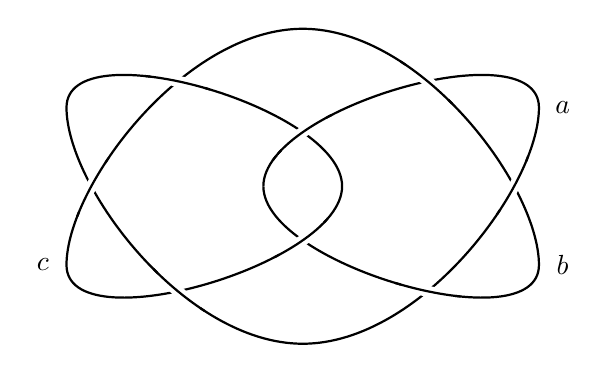
\begin{tikzpicture}
\begin{knot}[consider self intersections = true, clip width = 5, ignore endpoint intersections=false,
%draft mode = crossings,
flip crossing/.list={3, 5, 7}]
\strand[thick] (-0.5, 0) .. controls +(0, 1) and +(0, 1) .. (3, 1) .. controls +(0, -1) and +(1.5, 0) .. (0, -2) .. controls +(-1.5, 0) and +(0, -1) .. (-3, 1) .. controls +(0, 1) and +(0, 1) .. (0.5, 0) .. controls +(0, -1) and +(0, -1) .. (-3, -1) .. controls +(0, 1) and +(-1.5, 0) .. (0, 2) .. controls +(1.5, 0) and +(0, 1) .. (3, -1) .. controls +(0, -1) and +(0, -1) .. (-0.5, 0);
\end{knot}

\node at (3.3, 1) {$a$};
\node at (3.3, -1) {$b$};
\node at (-3.3, -1) {$c$};
\end{tikzpicture}
\caption{The knot $8_5$}
\label{fig:8-5}
\end{figure}

Note that by the Wirtinger algorithm, the reflection quotient (defined in Section \ref{subsec:reflection-quotient}) has a presentation
$$r(8_5) = \langle a, b, c\; | \; babc(ba)^2bc(ba)^4, babc(ba)^4cbabc(ab)^2a \rangle^{(2)}.$$
%TODO check this
These relations are satisfied in the Coxeter group
$$W = \langle a, b, c \; | \; (ab)^2, (ac)^3, (bc)^3 \rangle^{(2)}.$$
Thus, $W$ is a quotient of $\pi_1(S^3 \setminus 8_5)$.
\end{example}

Note that there exist presentations of the knot $8_5$, for example, any presentation involving more than three meridians, such that the above method does not work. It is thus difficult to prove in general that a fixed link $L$ does not admit a Coxeter quotient isomorphic to a specific Coxeter group $W$.

\subsection{Meridional Rank}
For a link $L \subset S^3$ we define its \textit{Coxeter rank}, abbreviated $\text{cr } L$, to be the maximal number $n$ such that $L$ has a Coxeter quotient of rank $n$. Abbreviating the meridional rank of $L$ by $\text{mr }L$ and the bridge index of $L$ by $\text{bi } L$, we have the following.

\begin{theorem}
Let $L \subset S^3$ be any link. Then we have the following chain of inequalities: $\textup{cr }L \leq \textup{mr }L \leq \textup{bi } L$.
\end{theorem}

\begin{proof}
The inequality $\textup{mr } L \leq \text{bi } L$ is well-known. Moreover, $\text{cr } L \leq \text{mr } L$, is a direct consequence of \cite[Lemma 2.1]{felikson2009}.
\end{proof}

Let us refer to a link $L \subset S^3$ that has a Coxeter quotient of rank $n = \text{bi } L$ as a \textit{Coxeter link}. Then we immadiately obtain:

\begin{corollary}\label{cor:coxeter-links-meridional-rank}
Coxeter links satisfy the meridional rank conjecture.
\end{corollary}

Another application of the techniques we have developed so far lies in the following.

\begin{theorem}\label{thm:connected-sums-coxeter-rank}
Let $K$ and $K'$ be knots. Then $\textup{cr } K\#K' \geq \textup{cr } K + \textup{cr } K' - 1$.
\end{theorem}

\begin{proof}
Let $W$ and $W'$ be Coxeter quotients of $K$ and $K'$, respectively. First we choose diagrams of $K$ and $K'$ such that the generators of $\pi(K)$ and $\pi(K')$ that get mapped to generating reflections of $W$ and $W'$ are diagram meridians. Let $s \in \pi(K)$ and $s' \in \pi(K')$ each be one of those diagram meridians.

Now observe that $\pi(K\#K')$ is of the form $\pi(K) * \pi(K') / ss'$. Thus, we can explicitly write down a Coxeter quotient of $K\#K'$ as follows. Let $\Gamma$ and $\Gamma'$ be the Coxeter graphs associated to $W$ and $W'$. Then there is a Coxeter quotient of $K\#K'$ with graph
\begin{center}
\begin{tikzpicture}
\draw[dashed] (0.85, 0.15) -- (0.15, 0.85);
\draw[dashed] (-0.15, 0.85) -- (-0.85, 0.15);
\draw (0.8, 0) -- (-0.8, 0);

\node at (0, 1) {$s$};
\node at (-1, 0) {$\Gamma$};
\node at (1, 0) {$\Gamma'$};
\node at (0, 0.2) {$\infty$};
\end{tikzpicture}
\end{center}
which has rank $\text{rk } W + \text{rk } W' - 1$. 
\end{proof}

\begin{corollary}
Knots of Coxeter rank two are prime.
\end{corollary}

\begin{proof}
This follows directly from the facts that bridge index one knots are prime and that the bridge index satisfies the same inequality, see Proposition \ref{prop:bridge-index-connected-sum}.
\end{proof}

\begin{corollary}
There are knots of arbitrarily high meridional rank.
\end{corollary}

\begin{proof}
Just take connected sums of your favorite non-trivial knot.
\end{proof}

\begin{corollary}
Connected sums of Coxeter knots are Coxeter knots.
\end{corollary}

\begin{proof}
Let $J, K \subset S^3$ be arbitrary knots. Then we have already shown that $\text{bi } J\#K = \text{bi } J + \text{bi } K - 1$ and $\text{cr } J\#K \leq \text{bi } J\#K$. If $J$ and $K$ are both Coxeter knots then equality immediately follows from Theorem \ref{thm:connected-sums-coxeter-rank}.
\end{proof}

\subsection{Rank Two Quotients}\label{subsec:rank-two}
Introduce Fox colorings and show how they are related to rank two Coxeter quotients. Introduce the determinant in the coloring sense and show how it is related to the Alexander polynomial.

\newpage

\section{Torus Knots}
The motto of this section will be that \textit{torus knots tend to admit few Coxeter quotients}. This is evident first in Section \ref{subsec:odd-weights}, where we show that an infinite class of torus knots does not admit any non-trivial Coxeter quotients, further adding to the well-known statement that \textit{knots of determinant one admit poor representation theory}.

\subsection{Preliminaries}
A particular result we will use over and over again is the following result concerning the bridge index of torus knots.

\begin{proposition}
Let $p, q$ be positive integers. Then we have that the bridge index of the $(p, q)$-torus knot is $p$. In particular, the $(p, q)$-torus knot does not admit any Coxeter quotients of rank higher than $p$.
\end{proposition}

\subsection{Odd Weights}\label{subsec:odd-weights}
As with many things when considering Torus knots, the qualitative features as far as Coxeter quotients go depend heavily on the weights $p, q$ of the $(p, q)$-torus knots. The reason for just considering odd weights lies in the fact that if $p$ and $q$ are odd, the $(p, q)$-torus knot has determinant one. The reason for this lies in the following well-known result.
%TODO cite

\begin{theorem}
Let $p, q$ be odd positive integers. Then the Alexander polynomial of $K = T(p, q)$ is
$$\Delta_K(t) = \frac{(t^{pq}-1)(t-1)}{(t^q-1)(t^p-1)}.$$
\end{theorem}

Because the determinant of a knot is its Alexander polynomial evaluated at $-1$, we immediately obtain the desired result.

\begin{corollary}
Let $p, q$ be odd. Then the $(p, q)$-torus has determinant one.
\end{corollary}

In Section \ref{subsec:rank-two} we have seen that this implies that torus knots with odd weights do not admit dihedral quotients. This brings us one step closer to the claim that torus knots with odd weights have very few Coxeter quotients. To illustrate our strategies, let us first fix $p = 3$.

\begin{theorem}\label{thm:p=3}
Let $q$ be an odd positive integer such that $q$ has no prime factor less than or equal to $5$. Then the $(3, q)$-torus knot does not admit any non-trivial Coxeter quotients.
\end{theorem}

Before proving this, we need a few lemmas.

\begin{lemma}
The only irreducible finite Coxeter groups with abelianization $\mathbb{Z}_2$ of rank three are $\mathbb{Z}_2 \times A_5$ and $S_4$.
\end{lemma}

\begin{proof}
This follows directly from the classification of finite irreducible Coxeter groups.
\end{proof}

\begin{lemma}
If $W$ is an infinite irreducible Coxeter group, then the center of $W$ is trivial.
\end{lemma}

%TODO proof

\begin{proof}[Proof of Theorem \ref{thm:p=3}]
It suffices to prove that $K = T(3, q)$ does not admit any rank three Coxeter quotients. Toward a contradiction, suppose $W$ is a Coxeter quotient of $K$ of rank three. Since $K$ is a knot we have that $W$ is irreducible. We will now consider two cases.

First, if $W$ is infinite, then $W$ has trivial center. Let $G = \pi(K)$ and consider the quotient map $\varphi: G \rightarrow W$. Recall that this means that for any meridian $m$ of $K$ we have that $\varphi(m)$ is a reflection in $W$. Since $\varphi$ is surjective we have that the center of $G$ is mapped into the center of $W$, and is thus sent to the identity. Recall that $G$ has a presentation
$$G = \langle a, b \; | \; a^3 = b^q \rangle$$
where $a$ and $b$ are meridian and longitude of the torus on which $K$ lies, respectively. Moreover, the center of $G$ is generated by the element $a^p = b^q$, which is a composition of an odd number of diagram meridians of $K$ since both $p$ and~$q$ are odd. But this is a contradiction: the image of $a^p = b^q$ in $W$ under~$\varphi$ is orientation-preserving because it is the identity, and orientation-reversing because it is the product of an odd number of reflections.

Finally, suppose $W$ is finite. Then $W$ is isomorphic to either $S_4$ or $\mathbb{Z}_2 \times A_5$ since $K$ is a knot. Note that $\varphi(b)$ has order dividing $q$, but by assumption $q$ has no divisor that is also a divisor of the order of $W$, which is either $24 = 2^3 \cdot 3$ or $120 = 2^3 \cdot 3 \cdot 5$.
%There are no infinite ones because $\pi(K)$ has non-trivial center and no finite ones because neither $S_4$ nor $\mathbb{Z}_2 \times A_5$ have elements of order the prime factor greater than or equal to $7$.
\end{proof}

In a very similar vein, we have to consider separately the case $p = 5$. First, we need to identify the finite irreducible Coxeter groups of rank five.

\begin{lemma}
The only irreducible finite Coxeter groups of rank five with abelianization $\mathbb{Z}_2$ are $S_6$ and a group of order $1920$.
\end{lemma}

With a very similar proof we obtain a very similar Theorem for $p = 5$.

\begin{theorem}
Let $q$ be an odd positive integer such that $q$ has no prime factor less than or equal to $5$. Then the $(5, q)$-torus knot does not admit any non-trivial Coxeter quotients.
\end{theorem}

Finally, we have a last look at the classification to see that for $p = 7$ we need to consider another exception: the group corresponding to the Coxeter graph $E_7$.

\begin{lemma}
The only irreducible finite Coxeter groups with abelianization $\mathbb{Z}_2$ of rank seven are $S_8$, a group of order $2^6 \cdot 7!$ and a group of order $72 \cdot 8!$.
\end{lemma}

\begin{theorem}
Let $q$ be an odd positive integer such that $q$ has no prime factor less than or equal to $7$. Then the $(7, q)$-torus knot does not admit any non-trivial Coxeter quotients.
\end{theorem}

Having gotten those special cases out of the way, we can now work with general odd $p$.

\begin{lemma}
Let $n \geq 9$ be an odd integer. Then the only irreducible finite Coxeter groups with abelianization $\mathbb{Z}_2$ of rank $n$ are of order $(n+1)!$ or $2^{n-1}\cdot n!$.
\end{lemma}

Seeing that all cases except $p = 3$ also fit in the statement arising from this, we can summarize everything else we have obtained in this section as follows.

\begin{theorem}
Let $5 \leq p < q$ be any odd coprime integers such that $q$ has no prime factor less than or equal to $p$. Then the $(p, q)$-torus knot does not admit any non-trivial Coxeter quotients.
\end{theorem}

\subsection{Close Weights}
This section contains an upshot showing that some torus knots in fact do have Coxeter quotients, namely the $(n, n + 1)$-torus knots.

\begin{example}[$n=4$]
Consider the braid representation of the $(4, 5)$-torus knot in Figure~\ref{fig:torus45}.

\begin{figure}[ht]
\centering
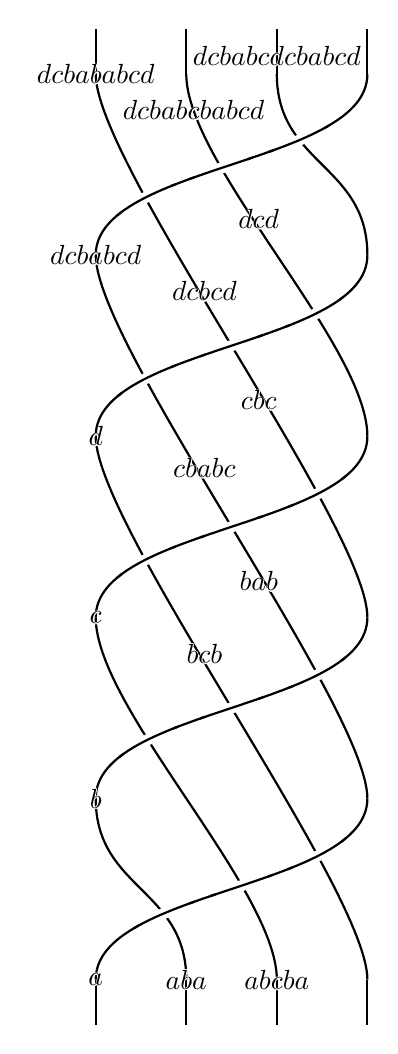
\begin{tikzpicture}[scale = 1.15]
\begin{knot}[clip width = 5, flip crossing/.list = {4, 5,6, 10, 11, 12}]
\strand[thick] (0, -0.5) -- (0, 0);
\strand[thick] (1, -0.5) -- (1, 0);
\strand[thick] (2, -0.5) -- (2, 0);
\strand[thick] (3, -0.5) -- (3, 0);

\strand[thick] (0, 0) .. controls +(0, 1) and +(0, -1) .. (3, 2);
\strand[thick] (1, 0) .. controls +(0, 1) and +(0, -1) .. (0, 2);
\strand[thick] (2, 0) .. controls +(0, 1) and +(0, -1) .. (0, 4);
\strand[thick] (3, 0) .. controls +(0, 1) and +(0, -1) .. (0, 6);

\strand[thick] (0, 2) .. controls +(0, 1) and +(0, -1) .. (3, 4);
\strand[thick] (0, 4) .. controls +(0, 1) and +(0, -1) .. (3, 6);
\strand[thick] (3, 2) .. controls +(0, 1) and +(0, -1) .. (0, 8);
\strand[thick] (3, 4) .. controls +(0, 1) and +(0, -1) .. (0, 10);

\strand[thick] (0, 6) .. controls +(0, 1) and +(0, -1) .. (3, 8);
\strand[thick] (0, 8) .. controls +(0, 1) and +(0, -1) .. (3, 10);

\strand[thick] (3, 6) .. controls +(0, 1) and +(0, -1) .. (1, 10);
\strand[thick] (3, 8) .. controls +(0, 1) and +(0, -1) .. (2, 10);



\strand[thick] (0, 10) -- (0, 10.5);
\strand[thick] (1, 10) -- (1, 10.5);
\strand[thick] (2, 10) -- (2, 10.5);
\strand[thick] (3, 10) -- (3, 10.5);
\end{knot}

\node at (0, 0) {\contour{white}{$a$}};
\node at (0, 2) {\contour{white}{$b$}};
\node at (0, 4) {\contour{white}{$c$}};
\node at (0, 6) {\contour{white}{$d$}};
\node at (0, 8) {\contour{white}{$dcbabcd$}};
\node at (0, 10) {\contour{white}{$dcbababcd$}};

\node at (1.2, 7.6) {\contour{white}{$dcbcd$}};
\node at (1.8, 8.4) {\contour{white}{$dcd$}};
\node at (1.8, 6.4) {\contour{white}{$cbc$}};
\node at (1.8, 4.4) {\contour{white}{$bab$}};
\node at (1.2, 5.65) {\contour{white}{$cbabc$}};
\node at (1.08, 9.6) {\contour{white}{$dcbabcbabcd$}};
\node at (2, 10.2) {\contour{white}{$dcbabcdcbabcd$}};

\node at (1, 0) {\contour{white}{$aba$}};
\node at (1.2, 3.6) {\contour{white}{$bcb$}};
\node at (2, 0) {\contour{white}{$abcba$}};
\end{tikzpicture}
\caption{The case $n = 4$}
\label{fig:torus45}
\end{figure}

Considering the first three strands we obtain a presentation of the reflection quotient of $K$, namely
$$r(K) = \langle a, b, c, d \; | \; adcbababcd, abadcbabcbabcd, abcbadcbabcdcbabcd \rangle^{(2)}.$$
The rules $a \mapsto (1 \; 2)$, $b \mapsto (2 \; 3)$, $c \mapsto (3 \; 4)$, $d \mapsto (4 \; 5)$ extend to a surjective homomorphism $r(K) \rightarrow S_5$, because all relators are mapped to the identity.
\end{example}

\begin{theorem}
Let $n \geq 2$ be an integer. Then the $(n, n+1)$-torus knot admit a Coxeter quotient isomorphic to $S_{n+1}$. In particular, $(n, n+1)$-torus knots are Coxeter.
\end{theorem}

\begin{proof} Similarly as before we consider the braid representation of the $(n, n+1)$-torus knot in Figure \ref{fig:torusnn+1}. The first $n-1$ strands give us the following defining relators.
\begin{itemize}
\item $s_1 s_n \cdots s_1 s_2 s_1 \cdots s_n$
\item $s_1s_2s_1 s_n \cdots s_1 s_2 s_3 s_2 s_1 \cdots s_n$
\item \dots
\item $s_1 \cdots s_{n-1} \cdots s_1 s_n \cdots s_1 \cdots s_n \cdots s_1 \cdots s_n$
\end{itemize}
These relations are all satisfied under the map $s_i \mapsto (i \;\;\; i+1)$. To see this, note that the general form of the above relators is
$$
s_1 \cdots s_i \cdots s_1 s_n \cdots s_1 \cdots s_{i + 1} \cdots s_1 \cdots s_n
$$
for $i = 1, \dots, n-1$. Compute $s_2s_1s_2s_1s_2 = s_1$,
and $s_js_1s_j = s_1$ for all $j \geq 3$. Thus, the first relator is the identity in $S_{n+1}$ by induction on $n$. Similarly it follows that all the other relators are zero in $S_{n+1}$.
%TODO do this
\end{proof}

\begin{figure}
\centering
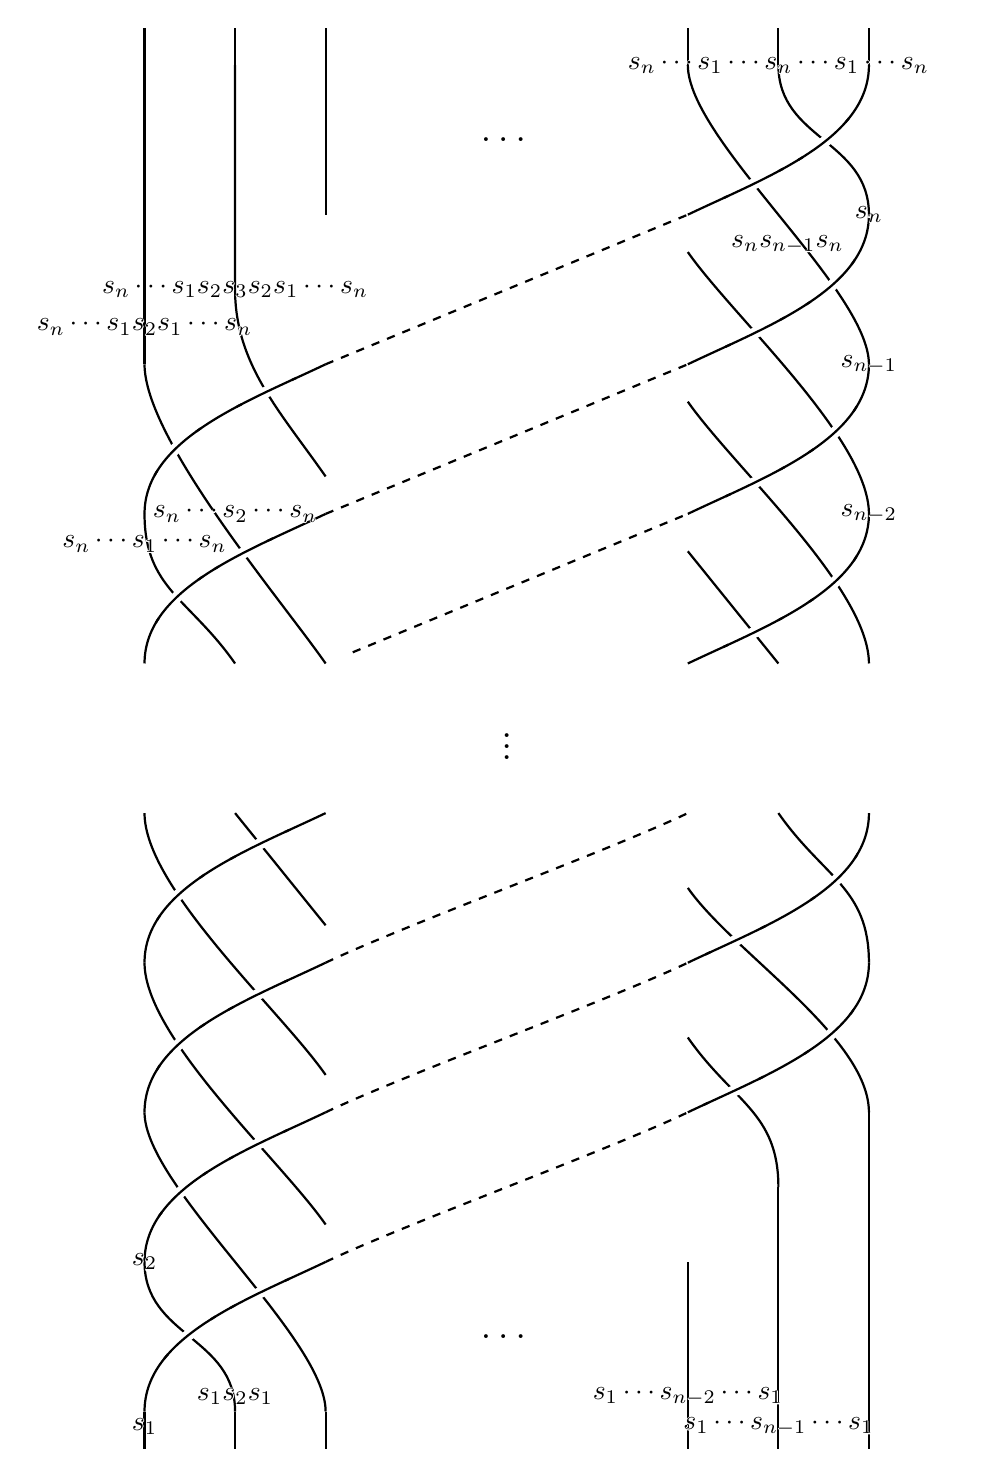
\begin{tikzpicture}[yscale=0.95, xscale=1.15]
\begin{knot}[clip width = 5]
\clip (-1.2, -0.5) rectangle (9.2, 18.5);
\strand[thick] (0, 0) .. controls +(0,1) and +(30:-1) .. (2, 2);
\strand[thick, dashed] (2, 2) .. controls +(30:1) and +(30:-1) .. (6, 4);
\strand[thick] (6, 4) .. controls +(30:1) and +(0, -1) .. (8, 6);
\strand[thick] (1, 0) .. controls +(0, 1) and +(0, -1) .. (0, 2);

\strand[thick] (0, 2) .. controls +(0,1) and +(30:-1) .. (2, 4);
\strand[thick, dashed] (2, 4) .. controls +(30:1) and +(30:-1) .. (6, 6);
\strand[thick] (6, 6) .. controls +(30:1) and +(0, -1) .. (8, 8);
\strand[thick] (2, 0) .. controls +(0, 1) and +(0, -1) .. (0, 4);

\strand[thick] (0, 4) .. controls +(0,1) and +(30:-1) .. (2, 6);
\strand[thick, dashed] (2, 6) .. controls +(30:1) and +(30:-1) .. (6, 8);

\strand[thick] (0, 6) .. controls +(0, 1) and +(30:-1) .. (2, 8);

\strand[thick] (6, 0) -- (6, 2);
\strand[thick] (7, 0) -- (7, 3);
\strand[thick] (7, 3) .. controls +(0, 1) and +(120:-1) .. (6, 5);
\strand[thick] (8, 0) -- (8, 4);
\strand[thick] (8, 4) .. controls +(0, 1) and +(120:-1) .. (6, 7);
\strand[thick] (8, 6) .. controls +(0, 1) and +(120:-1) .. (7, 8);

\strand[thick] (2, 6.5) -- (1, 8);
\strand[thick] (2, 2.5) .. controls +(120:1) and +(0, -1) .. (0, 6);
\strand[thick] (2, 4.5) .. controls +(120:1) and +(0, -1) .. (0, 8);

\strand[thick] (0, 10) .. controls +(0,1) and +(30:-1) .. (2, 12);
\strand[thick, dashed] (2, 12) -- (6, 14);
\strand[thick] (6, 14) .. controls +(30:1) and +(0, -1) .. (8, 16);


\strand[thick] (0, 12) .. controls +(0,1) and +(30:-1) .. (2, 14);
\strand[thick, dashed] (2, 14) -- (6, 16);
\strand[thick] (6, 16) .. controls +(30:1) and +(0, -1) .. (8, 18);
\strand[thick] (1, 10) .. controls +(120:1) and +(0, -1) .. (0, 12);
\strand[thick] (2, 10) .. controls +(120:1) and +(0, -1) .. (0, 14);
\strand[thick] (0, 14) -- (0, 18);

\strand[thick] (2, 12.5) .. controls +(120:1) and +(0,-1) .. (1, 15) -- (1, 18);
\strand[thick] (2, 16) -- (2, 18);

\strand[thick, dashed] (2.3, 10.15) -- (6, 12);
\strand[thick] (6, 12) .. controls +(30:1) and +(0, -1) .. (8, 14);
\strand[thick] (6, 10) .. controls +(30:1) and +(0, -1) .. (8, 12);

\strand[thick] (8, 16) .. controls +(0, 1) and +(0, -1) .. (7, 18);
\strand[thick] (8, 14) .. controls +(0, 1) and +(0, -1) .. (6, 18);
\strand[thick] (8, 12) .. controls +(0, 1) and +(120:-1) .. (6, 15.5);
\strand[thick] (8, 10) .. controls +(0, 1) and +(120:-1) .. (6, 13.5);
\strand[thick] (7, 10) -- (6, 11.5);

%tails
\strand[thick] (0, 18) -- +(0, 0.5);
\strand[thick] (1, 18) -- +(0, 0.5);
\strand[thick] (2, 18) -- +(0, 0.5);
\strand[thick] (6, 18) -- +(0, 0.5);
\strand[thick] (7, 18) -- +(0, 0.5);
\strand[thick] (8, 18) -- +(0, 0.5);

\strand[thick] (0, 0) -- +(0, -0.5);
\strand[thick] (1, 0) -- +(0, -0.5);
\strand[thick] (2, 0) -- +(0, -0.5);
\strand[thick] (6, 0) -- +(0, -0.5);
\strand[thick] (7, 0) -- +(0, -0.5);
\strand[thick] (8, 0) -- +(0, -0.5);
\end{knot}

\node at (4, 1) {\Large{$\dots$}};
\node at (4, 17) {\Large{$\dots$}};
\node at (4, 9) {\Large{$\vdots$}};

\node at (0, -0.2) {\contour{white}{$s_1$}};
\node at (0, 2) {\contour{white}{$s_2$}};
%\node at (0, 4) {\contour{white}{$s_3$}};

\node at (1, 0.2) {\contour{white}{$s_1s_2s_1$}};
%\node at (1, 2) {\contour{white}{$s_2s_3s_2$}};
%\node at(2, 0.2) {\contour{white}{$s_1s_2s_3s_2s_1$}};
\node at (6, 0.2) {\contour{white}{$s_1 \dotsm s_{n-2} \dotsm s_1$}};
\node at (7, -0.2) {\contour{white}{$s_1 \dotsm s_{n-1} \dotsm s_1$}};
%\node at (0, 10) {\contour{white}{$s_n$}};
\node at (8, 14) {\contour{white}{$s_{n-1}$}};
\node at (8, 12) {\contour{white}{$s_{n-2}$}};
%\node at (8, 10) {\contour{white}{$s_{n-3}$}};
%\node at (7.5, 13.6) {\contour{white}{$s_{n-1}s_{n-2}s_{n-1}$}};
%\node at (6.4, 13.2) {\contour{white}{$s_{n-1}s_{n-2}s_{n-3}s_{n-2}s_{n-1}$}};

\node at (8, 16) {\contour{white}{$s_n$}};
\node at (7.1, 15.6) {\contour{white}{$s_ns_{n-1}s_n$}};
\node at (0, 11.6) {\contour{white}{$s_n\dotsm s_1 \dotsm s_n$}};
\node at (1, 12) {\contour{white}{$s_n \dotsm s_2 \dotsm s_n$}};

\node at (0, 14.5) {\contour{white}{$s_n \dotsm s_1 s_ 2 s_ 1 \dotsm s_n$}};
\node at (1, 15) {\contour{white}{$s_n \dotsm s_1 s_ 2 s_3 s_2 s_1 \dotsm s_n$}};
\node at (7, 18) {\contour{white}{$s_n \dotsm s_1 \dotsm s_n \dotsm s_1 \dotsm s_n$}};

\end{tikzpicture}
\caption{The braid representation of the $(n, n+ 1)$-torus knot}
\label{fig:torusnn+1}
\end{figure}

\subsection{Other Weights}
We are nowhere close to understanding what happens in the cases not covered above. For example, the $(3, 5)$- and the $(3, 25)$-torus knots both have a $\mathbb{Z}_2 \times A_5$-quotient. Moreover, all known Coxeter quotients of Torus knots and links are finite, which is not clear from the above arguments.

\newpage

\section{Pretzel Knots}
\subsection{Preliminaries}
\subsection{A Coxeter Quotient}
\begin{theorem}\label{thm:pretzel-links-are-coxeter}
Pretzel links are Coxeter. 
\end{theorem}

\begin{proof} First consider the situation of how assigning letters to meridians propagates in 2-braids in Figure \ref{fig:elementary-twists}.
\begin{figure}[ht]
\centering
\begin{minipage}{.5\textwidth}
\centering

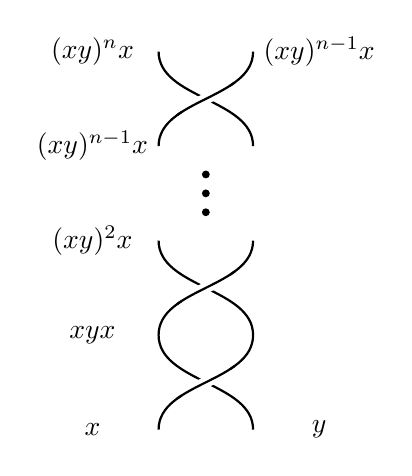
\begin{tikzpicture}[scale = 0.6]
\begin{knot}[clip width = 5, flip crossing = 2]

\strand[black, thick] (0, 0) .. controls +(0, 1) and +(0, -1) .. (2, 2) .. controls +(0, 1) and +(0, -1) .. (0, 4);

\strand[black, thick] (2, 0) .. controls +(0, 1) and +(0, -1) .. (0, 2) .. controls +(0, 1) and +(0, -1) .. (2, 4);

\strand[black, thick] (0, 6) .. controls +(0, 1) and +(0, -1) .. (2, 8);

\strand[black, thick] (2, 6) .. controls +(0, 1) and +(0, -1) .. (0, 8);

\end{knot}

\node at (1, 4.6) [circle, fill, inner sep=1pt]{};
\node at (1, 5) [circle, fill, inner sep=1pt]{};
\node at (1, 5.4) [circle, fill, inner sep=1pt]{};


\node at (-1.4, 0) {$x$};
\node at (3.4, 0) {$y$};
\node at (-1.4, 2) {$xyx$};
\node at (-1.4, 4) {$(xy)^2x$};
\node at (-1.4, 6) {$(xy)^{n-1}x$};
\node at (-1.4, 8) {$(xy)^nx$};
\node at (3.4, 8) {$(xy)^{n-1}x$};

\end{tikzpicture}

\end{minipage}%
\begin{minipage}{.5\textwidth}
\centering
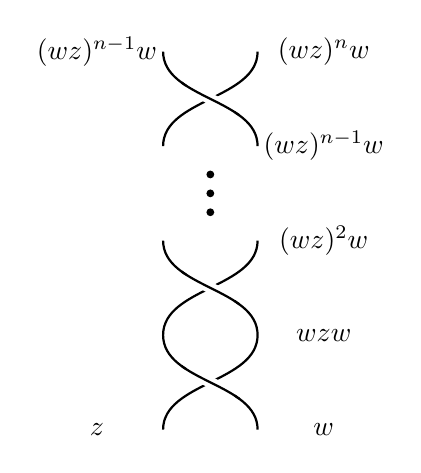
\begin{tikzpicture}[scale = 0.6]
\begin{knot}[clip width = 5, flip crossing/.list = {1, 3}]

\strand[black, thick] (0, 0) .. controls +(0, 1) and +(0, -1) .. (2, 2) .. controls +(0, 1) and +(0, -1) .. (0, 4);

\strand[black, thick] (2, 0) .. controls +(0, 1) and +(0, -1) .. (0, 2) .. controls +(0, 1) and +(0, -1) .. (2, 4);


\strand[black, thick] (0, 6) .. controls +(0, 1) and +(0, -1) .. (2, 8);

\strand[black, thick] (2, 6) .. controls +(0, 1) and +(0, -1) .. (0, 8);

\end{knot}


\node at (1, 4.6) [circle, fill, inner sep=1pt]{};
\node at (1, 5) [circle, fill, inner sep=1pt]{};
\node at (1, 5.4) [circle, fill, inner sep=1pt]{};

\node at(-1.4, 0) {$z$};
\node at(3.4, 0) {$w$};
\node at (3.4, 2) {$wzw$};
\node at (3.4, 4) {$(wz)^2w$};
\node at (3.4, 6) {$(wz)^{n-1}w$};
\node at (3.4, 8) {$(wz)^n w$};
\node at (-1.4, 8) {$(wz)^{n-1}w$};

\end{tikzpicture}

\end{minipage}
\caption{The relations for 2-braids}
\label{fig:elementary-twists}
\end{figure}

Now note that assigning letters of meridians as in the local situation in Figure \ref{fig:local-picture-pretzel-link}, we in fact obtain a generating set of the link group $\pi(P(l_1, \dots, l_k))$.


\begin{figure}[ht]
\centering
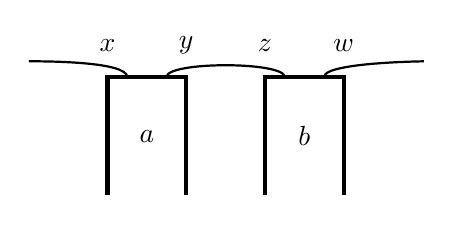
\begin{tikzpicture}
\draw[ultra thick] (0, -1.5) -- (0, 0) -- (1, 0) -- (1, -1.5);
\draw[ultra thick] (2, -1.5) -- (2, 0) -- (3, 0) -- (3, -1.5);

\begin{knot}
\strand[thick] (0.25, 0) .. controls +(0, 0.2) and +(0.2, 0) .. (-1, 0.2);
\strand[thick] (0.75, 0) .. controls +(0, 0.2) and +(0, 0.2) .. (2.25, 0);
\strand[thick] (2.75, 0) .. controls +(0, 0.2) and +(0.2, 0) .. (4, 0.2);
\end{knot}

\node at (0, 0.4) {$x$};
\node at (1, 0.4) {$y$};
\node at (2, 0.4) {$z$};
\node at (3, 0.4) {$w$};

\node at (0.5, -0.75) {$a$};
\node at (2.5, -0.75) {$b$};
\end{tikzpicture}

\caption{A local picture}
\label{fig:local-picture-pretzel-link}
\end{figure}

Putting these 2-braids together as in Figure \ref{fig:local-picture-pretzel-link} we obtain the following relation in the knot group from the requirement that $y = z$ according as to whether $a$ and $b$ are positive or negative:

\begin{itemize}
\item If both $a$ and $b$ are positive, then we obtain $(xy)^{a-1}x = (yw)^by.$
\item If $a$ is positive and $b$ is negative, we obtain $(xy)^{a-1}x = (wy)^{-b+1}w$.
\item If $a$ is negative and $b$ is positive, we obtain $(yx)^{-a}y = (yw)^b y$.
\item If both $a$ and $b$ are negative, then we obtain $(yx)^{-a}y = (wy)^{-b+1}w$.
\end{itemize}

All these relations follow from the Coxeter relations $(xy)^{|a|} = (yw)^{|b|} = 1$. Assigning generators as in Figure \ref{fig:local-picture-pretzel-link} we get a quotient of the desired form.
\end{proof}

This Theorem and its proof have some consequences that, although well-known, still require some work to prove. So it is worth it to state them with proofs in our setting.

\begin{corollary}
Pretzel links satisfy the meridional rank conjecture.
\end{corollary}

\begin{proof}
This is just Corollary \ref{cor:coxeter-links-meridional-rank}.
\end{proof}

%TODO
\begin{question}
Is there more to deduce?
\end{question}

It might be worth pointing out that the explicit Coxeter quotient obtained is described by the matrix

$$
\renewcommand\arraystretch{1.2}
M = \left( \begin{matrix}
1 & l_1 & \infty & \cdots & \cdots &\cdots & \infty & l_n \\
l_1 & 1 & l_2 & \infty & \cdots & \cdots & \infty & \infty \\
\infty & l_2 & 1 & l_3 & \infty &\cdots & \infty & \infty \\
\vdots & \infty  & l_3 & 1 & \ddots & \ddots & \vdots & \vdots \\
\vdots & \vdots & \infty & \ddots & \ddots & \ddots & \infty & \vdots \\
\vdots & \vdots & \vdots & \ddots &\ddots & 1 & \l_{n-2} & \infty \\
\infty & \infty & \infty & \cdots & \infty & l_{n-2} & 1 & l_{n-1} \\
l_n & \infty & \infty & \cdots & \cdots & \infty  & l_{n-1} & 1
\end{matrix} \right).$$

\newpage

\section{Questions}

\bibliography{biblio}
\bibliographystyle{plain}

\end{document}